\documentclass{beamer}
\usepackage{verbatim}
\usetheme{Boadilla}
\title
{Technical Runs: Partition configuration}
\author[Argyris Zardilis]
{Argyris Zardilis \inst{}}
\institute[CERN]
{
  \inst{}
  CERN
}
\date[DAQ/HLT meeting, 15/08/2013]
{DAQ/HLT meeting, 15 August 2013}

\begin{document}

\frame{\titlepage}

\begin{frame}
  \frametitle{Motivation}
  \begin{itemize}
    \item Large amount of information in a partition, hard to create its configuration manually \\
      \textbf{Solution}: Use a tool that automates all or part of the process

    \item \textit{PartitionMaker}: fully featured configuration generation
      \begin{itemize}
        \item Depends heavily on design and schema
        

        \item Difficult to keep up to date with constant schema changes during design evolution
      \end{itemize}


    \item Last Technical Run: need to create partition of different flavours to test different components
      of the system and their combinations.

    \item Manual partition configuration generation laborious and time-consuming

    \item Minimise time loss during TR
  \end{itemize}
  
\end{frame}


\begin{frame}
  \frametitle{Solution}
  \begin{itemize}
    \item Created a command-line script that automates generation process

    \item Started as a temporary solution for TR2 but since grew to a more complete
      and configurable command-line tool akin to \textit{PartitionMaker}.

    \item By no means as complete or comprehensive but covers basic use cases

    \item Build on top of config and Python DAL package to get access to base classes defined in OKS schema 

    \item Also uses pm.project from \textit{PartitionMaker} to get a convenient handle to the config db

  \end{itemize}
\end{frame}


\begin{frame}
 \frametitle{Solution schematically}
 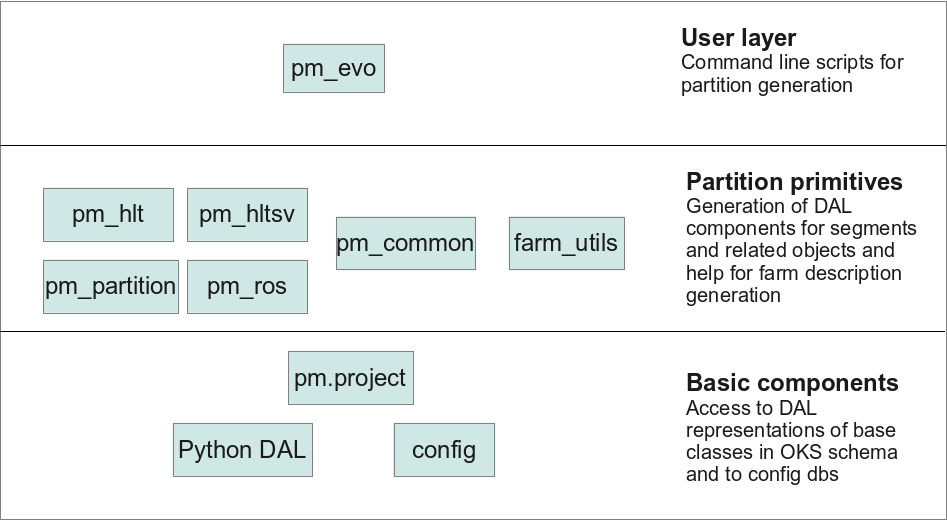
\includegraphics[height=8cm,width=12cm]{images/partition_maker_layers.png}
 
\end{frame}


\begin{frame}
\frametitle{Partition generation flow}
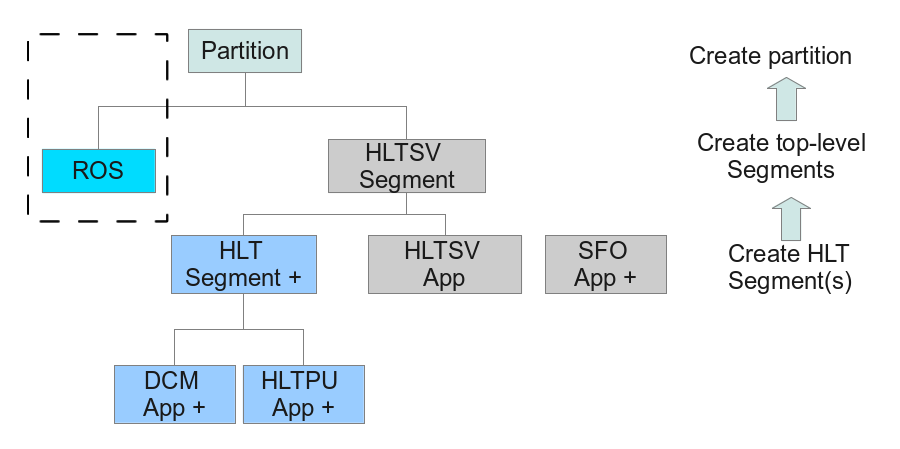
\includegraphics[height=5.5cm,width=12cm]{images/generation_flow.png} \\
Bottom-up approach. Start from primitive segments(don't contain other segments) and then pass their handle to their container segments and so on.
\end{frame}


\begin{frame}
 \frametitle{Capabilities}
 \begin{itemize}
   \item Create localhost or multihost partitions in testbed/P1
     \begin{itemize}
       \item farm description loaded from user provided python dictionary (a la \textit{PartitionMaker})
     \end{itemize}
   \item Create standard partitions: only DCMs, only HLTPUs
     \begin{itemize}
       \item customisable through command line parameters
     \end{itemize}

   \item Create standalone, pluggable HLTSV segment
     
   \item Doesn't handle ROS segment generation
     \begin{itemize}
       \item Not needed during TR (standard ROS segment)
     \end{itemize}

   \item Also includes configuration for standard monitoring applications
   \begin{itemize}
     \item Histogram/IS Gatherer
   \end{itemize}
     
   \item Other configurable parameters: extra includes, data networks, repository root

 \end{itemize}
 
\end{frame}


\begin{frame}
  \frametitle{Example usage}
  Create a DCM only partition with a provided python file 'farm\_gen' containing farm
  description with partition name 'az\_test' and repository root my home directory:
  \begin{itemize}
    \item \texttt{tdaq\_python pm\_evo.py -p az\_test -f farm\_gen --dcm-only -r tbed/user/azardili/installed}

  \end{itemize}

    Create a DCM/HLTPU partition with a provided python file 'farm\_gen' containing farm
  description with partition name 'az\_test' with PuDummy.data.xml as extra include:
  \begin{itemize}
    \item \texttt{tdaq\_python pm\_evo.py -p az\_test -f farm\_gen -I PuDummy.data.xml}

  \end{itemize}
\end{frame}


\begin{frame}
  \frametitle{Conclusions}
  \framesubtitle{and Future Work}
  \begin{itemize}
    \item A crude version proved useful for some use-cases in TR2.

    \item Short term plans: Use new polished version more extensively
      in next TR or for tests in testbed
      \begin{itemize}
        \item Bonus: can be used by anyone now and it doesn't require knowledge of the
          code anymore!
      \end{itemize}

    \item Use feedback from usage experience for subsequent development/evolution of \textit{PartitionMaker}
     \begin{itemize}
       \item Use-cases for new DF/run control/monitoring

       \item New requirements

      \end{itemize}
     
    \item Current version lives in a private git repo on my public afs
      partition which you can clone:
      \begin{itemize}
        \item \texttt{/afs/cern.ch/user/a/azardili/public/partition\_maker}
      \end{itemize}
  \end{itemize}
\end{frame}


\end{document}
